\documentclass[11pt, oneside]{article}   	% use "amsart" instead of "article" for AMSLaTeX format
\usepackage{geometry}                		% See geometry.pdf to learn the layout options. There are lots.
\geometry{letterpaper}                   		% ... or a4paper or a5paper or ... 
%\geometry{landscape}                		% Activate for rotated page geometry
%\usepackage[parfill]{parskip}    		% Activate to begin paragraphs with an empty line rather than an indent
\usepackage{graphicx}				% Use pdf, png, jpg, or eps§ with pdflatex; use eps in DVI mode
\usepackage{grffile}                                   % Searches for welknown image extensions. graphicx uses the first dot it finds ... which doesn't help when we have long filenames with dots in
								% TeX will automatically convert eps --> pdf in pdflatex		
\usepackage{amssymb}
\usepackage{setspace,caption}
\usepackage[titletoc,title]{appendix}
\usepackage[linkcolor=blue,colorlinks=true,urlcolor=blue,citecolor=black]{hyperref}
\usepackage{pdfpages}

\title{AMMA-2050 Atlas of Climate Metrics}
%\author{Rory Fitzpatrick, Conni Klein, Andrew Hartley, Famien Moise\\Adama Bamba, Nana Ama Browne Klutse, N'Datchoh Evelyne Toure, Oumar Konte\\Siny N'Doye, Youssouph Sane, Dave Rowell, Serge Janicot}

%\date{v0.1 May 2017}							% Activate to display a given date or no date

\newpage

\begin{document}

\maketitle
\tableofcontents
\thispagestyle{empty} 
\listoffigures

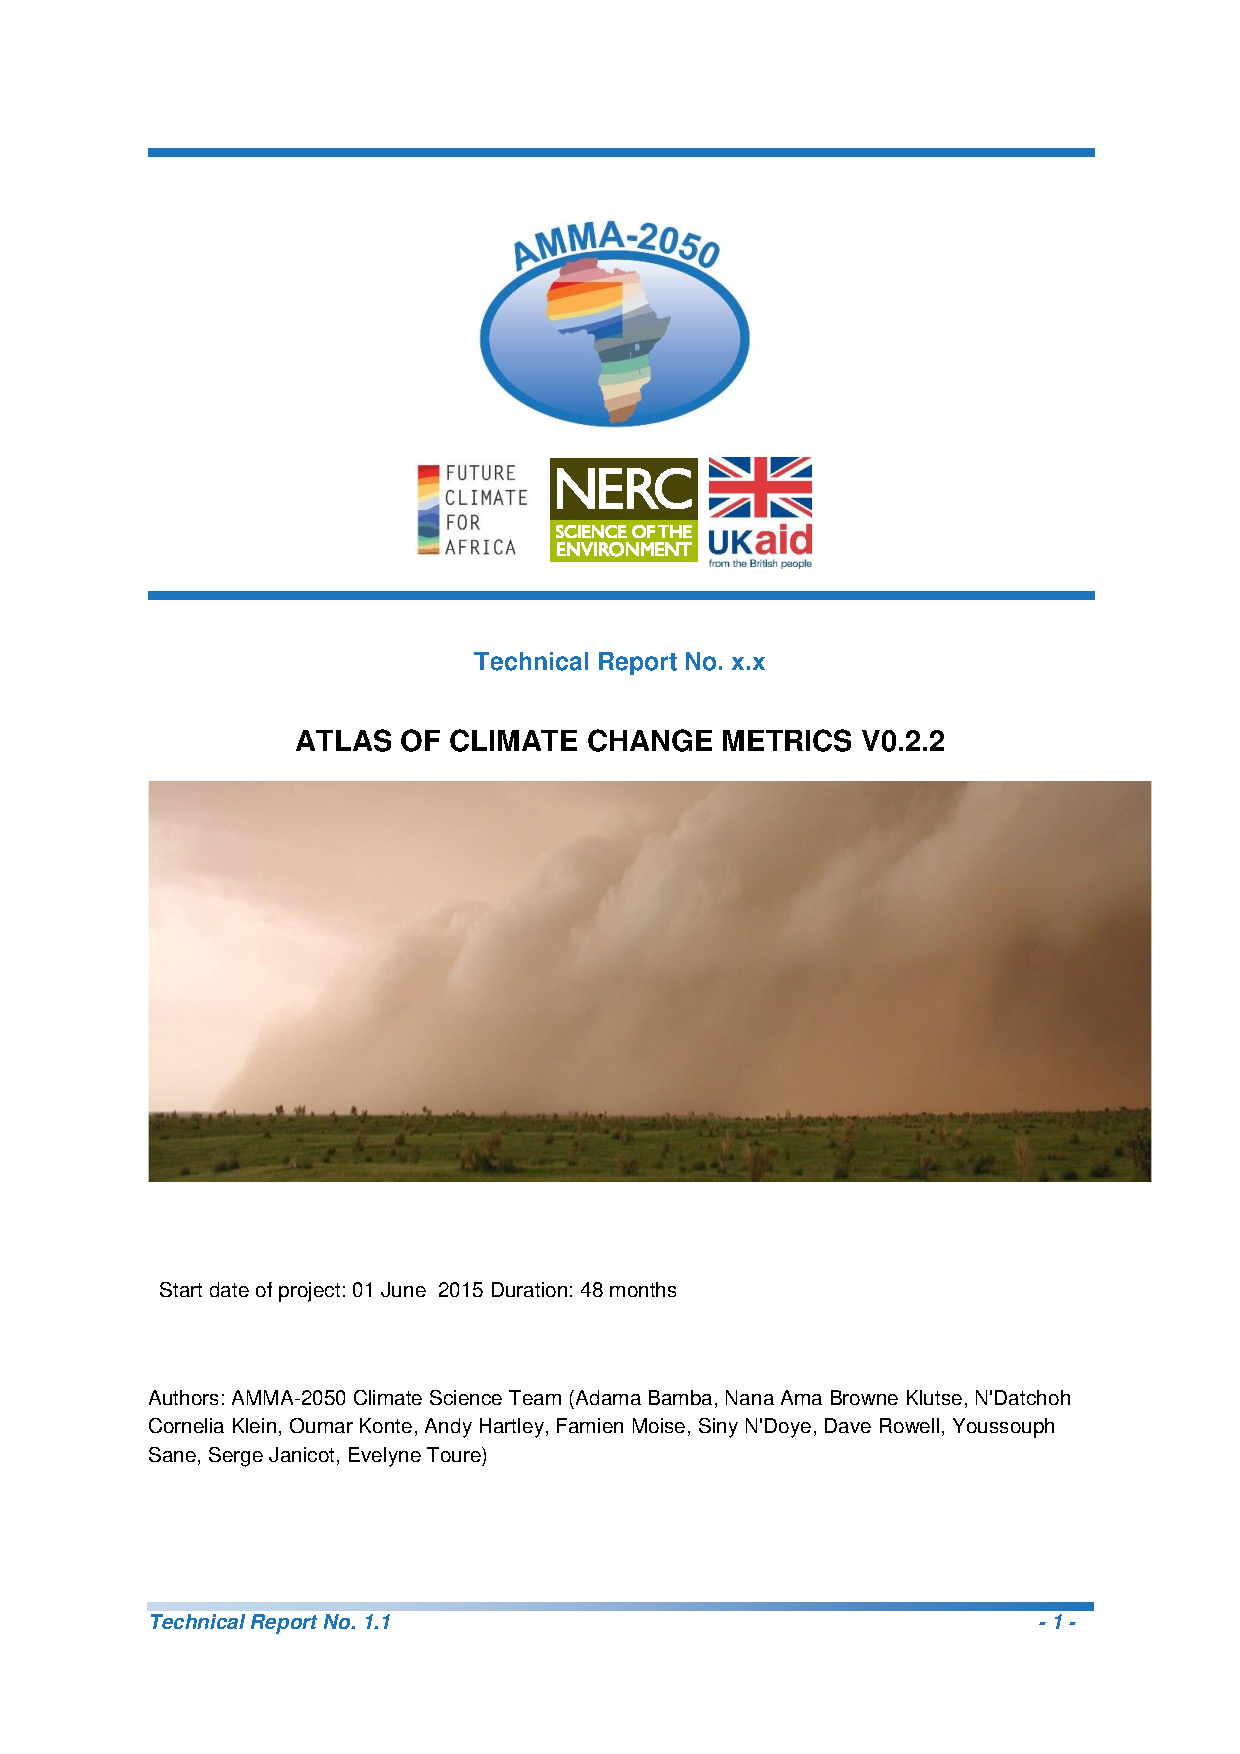
\includepdf[pages={1,2}]{AMMA2050_atlas_coverpage_v0p2p2.pdf}

\section{Introduction} \label{sec:intro}

This atlas has been created to provide relevant and up-to-date information on projected climate change in West Africa by the 2050s, crucially incorporating information on the modelling uncertainties that still persist. It forms a series of atlases, each addressing a specific region, month or season, and dataset version.

These atlases have been created by a team of African and European climate scientists within the FCFA AMMA-2050 project. The project aims to improve understanding of how the West African monsoon will be affected by climate change in the coming decades and to enhance the capacity of West African societies to prepare and adapt. 

Our aim is to present maps and graphs of the changes and uncertainties in climate metrics that are relevant to stakeholders. We use the term 'climate metric' to describe a statistical measure of an aspect of climate that may change in the future, and that is thought to be relevant for assessing the effects of high impact weather and climate in West Africa. These climate metrics were chosen by groups of AMMA-2050 impacts scientists, in consultation with the project's climate scientists. We have also taken some feedback from stakeholders.

The audience for this atlas is envisaged to be:

\begin{itemize}
  \item \textbf{\textit{Climate change impact scientists}}, principally from the hydrological and agricultural communities. Suitably presented information on the changes and uncertainties in the most relevant aspects of West African climate should help interpret the output of impacts models, such as changes in crop yields, flooding frequency, etc.
  \item \textbf{\textit{Technical experts}} in government ministries and local, national, regional and international bodies, engaged in sectors and services directly impacted by climate variability and change. This contributes to informed resource management decisions based on the plausible range of future climate outcomes. They will likely benefit from an understanding of the climate change context behind the outputs of impact modelling that AMMA-2050 will provide, such as changes in crop yields and flooding frequency. A key outcome of AMMA-2050 is the development of appropriate communication tools to help stakeholders understand the predicted impacts and uncertainties for each of their sectors. This atlas is not seen as one of these primary communication tools, but rather as an optional supplementary technical source of information that those stakeholders who have some understanding of modelling climate change may choose to use.
\end{itemize}

Climate model data was sourced from the CMIP5 archive (which is also that used in the IPCC 5th Assessment Report), and then post-processed at IPSL to disaggregate the projections to a 0.5\textdegree grid (a process sometimes called 'downscaling'). Two versions are available (used in separate atlases), with and without bias correction, a process by which discrepancies between the historical model simulations and observations are corrected. Further details of these techniques are being prepared for publication.

The climate metrics analysed here are the majority of those published in AMMA-2050's Technical report No. 1. Exceptions are evapotranspiration and humidity-based metrics (not yet bias-corrected and disaggregated), wet season duration (awaiting a definition), seasonal mean temperature from onset date (over-sensitive to onset definition + coding complexities), and 4 medium-priority metrics (drought severity, max seasonal no. of consecutive dry days, diurnal temperature range, and number of wind events greater than 70km/hr; all due to coding complexities).


%InsertHere

%\begin{appendices}
%\include{MetricDescriptions}
%\end{appendices}

\bibliographystyle{abbrvnat}
\bibliography{atlasBibliography}

\end{document}  
